\chapter{疫情数据的获取与存储}
\section{数据的获取}

通过分析腾讯新冠肺炎最新动态网站https://news.qq.com/zt2020/page/feiyan.htm,并使用开发者工具对其进行分析,可以得到腾讯疫情数据的接口如下。

\begin{figure}[H]
    \centering
    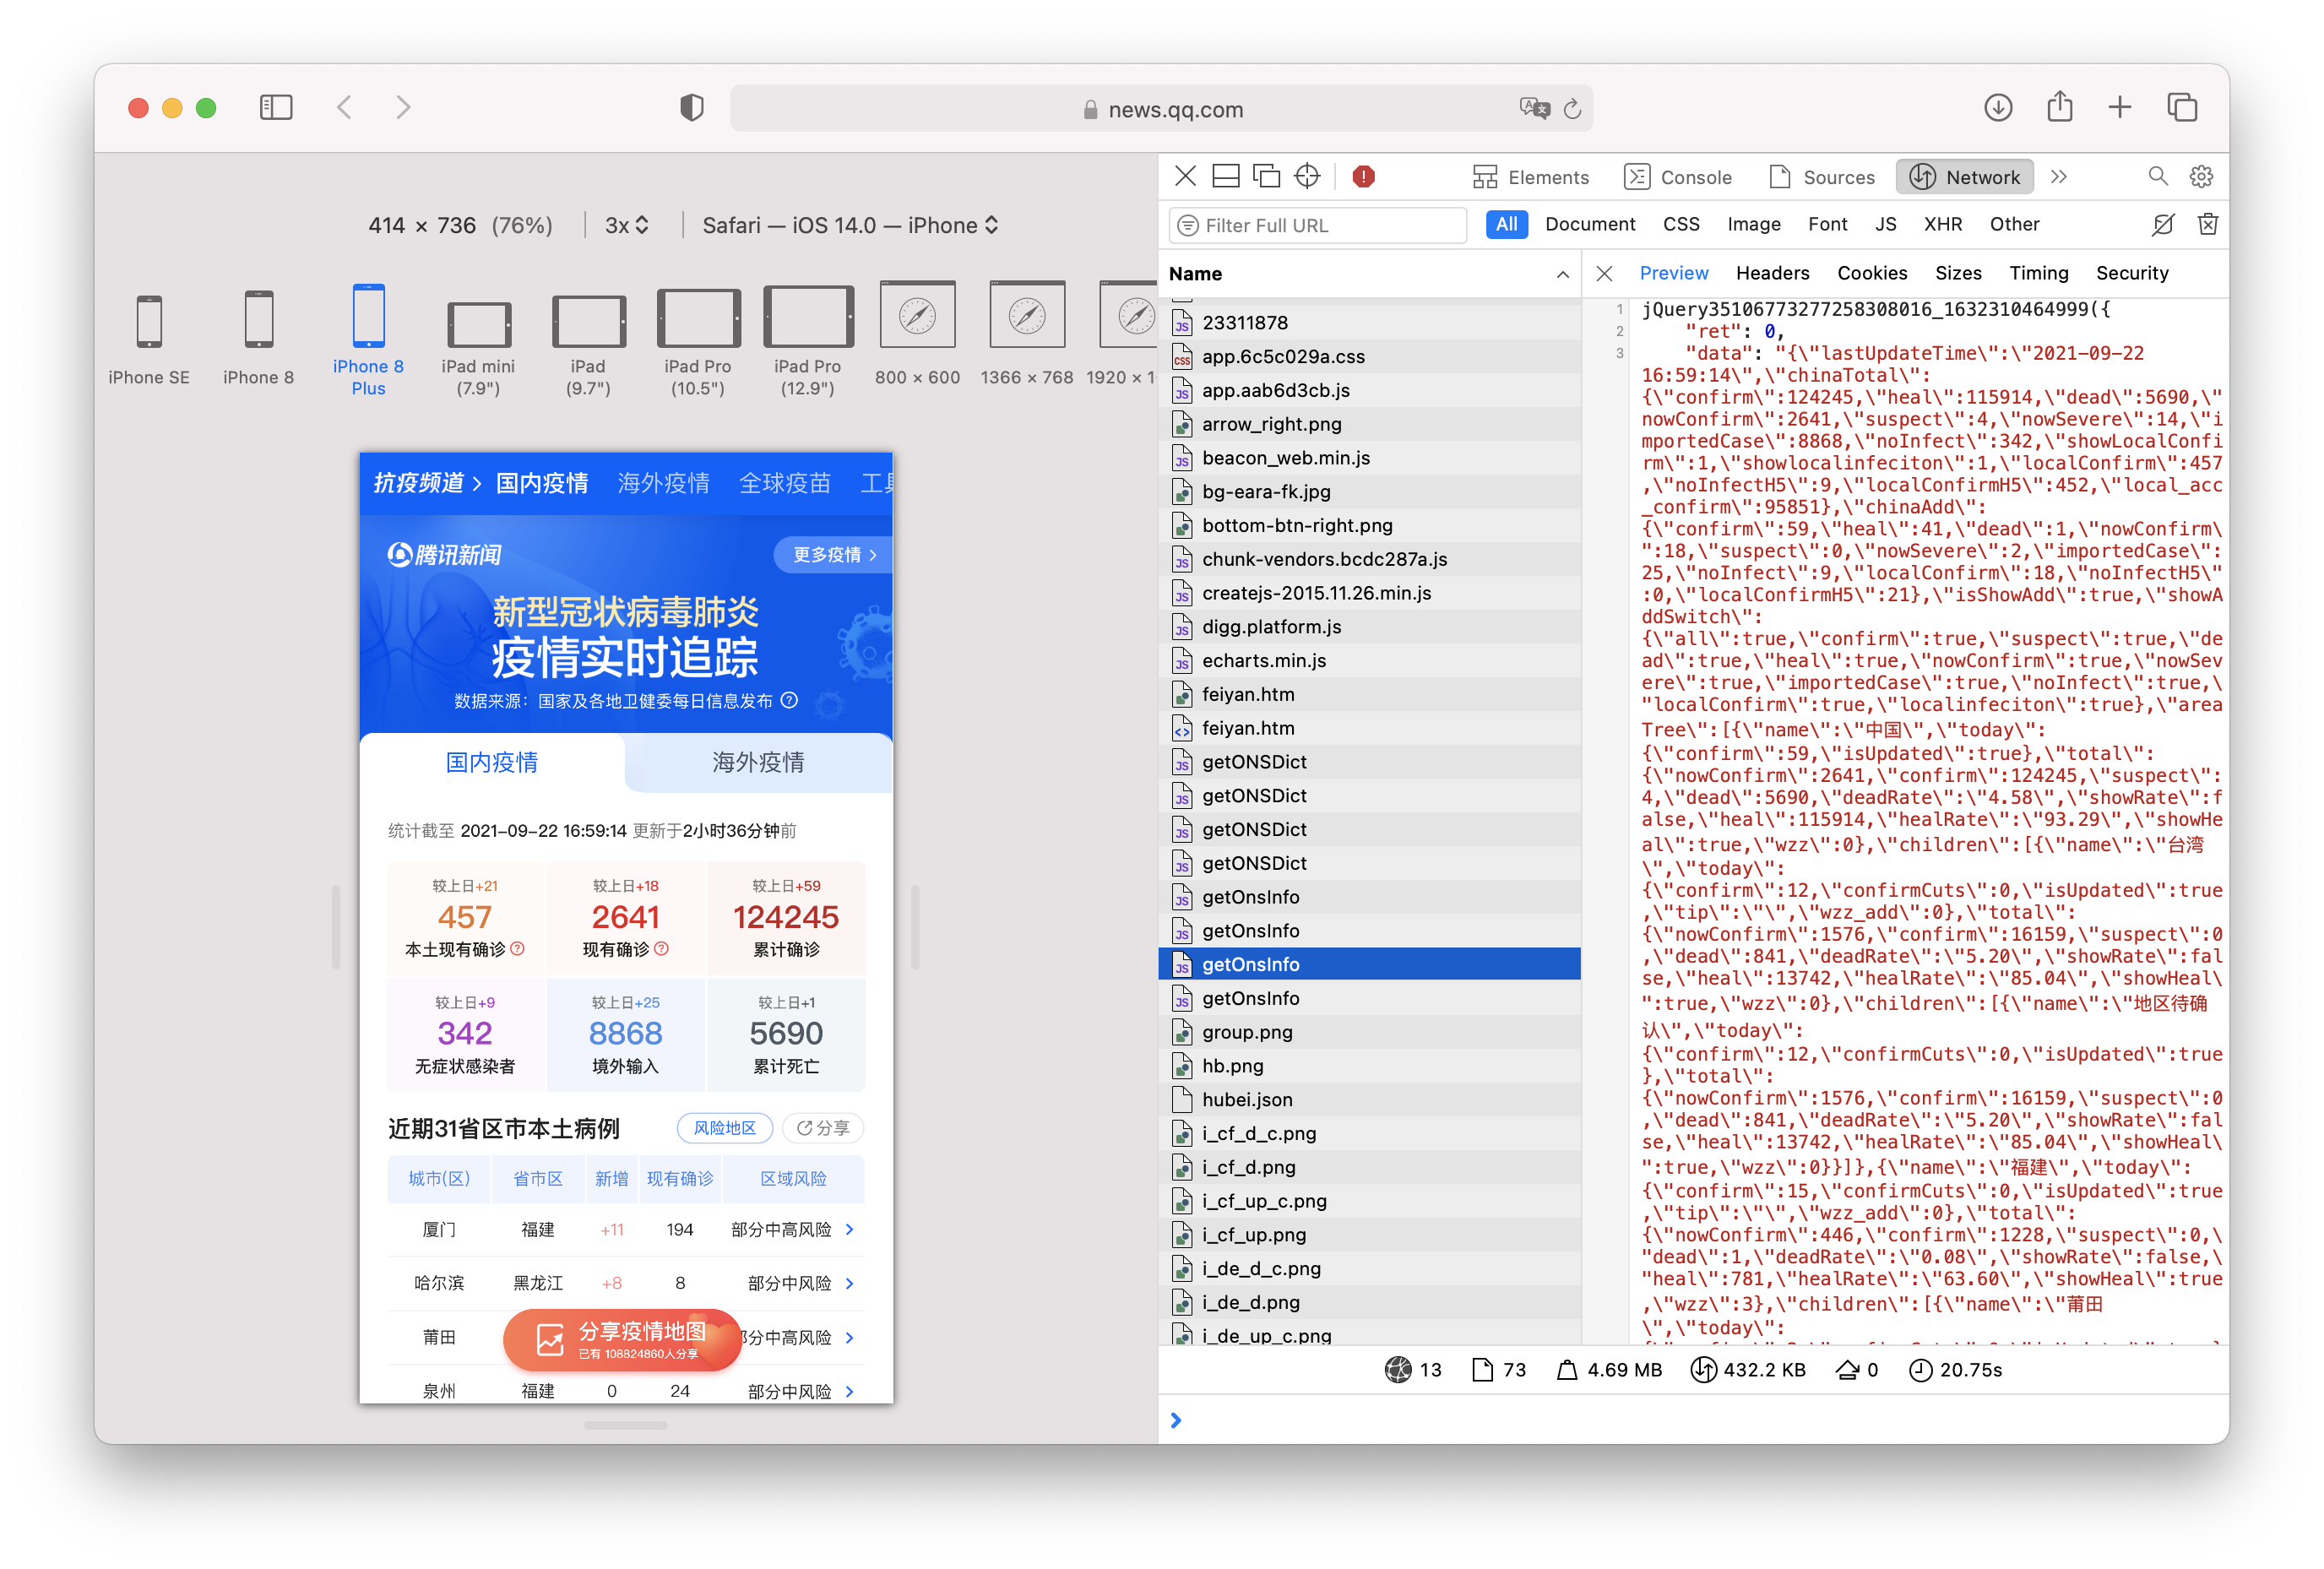
\includegraphics[width=0.8\textwidth]{t3}
    \bicaption{查看腾讯新闻疫情数据网站network情况}{Check Tencent News Epidemic Data Website Network Status}
    \label{fig:t3}
\end{figure}

之后,使用Python的requests库请求数据接口,然后解析json数据,将数据转换为字典类型,代码如下。

\lstset{
 columns=fixed,       
 numbers=left,                                        % 在左侧显示行号
 numberstyle=\tiny\color{gray},                       % 设定行号格式
 frame=none,                                          % 不显示背景边框
 backgroundcolor=\color[RGB]{245,245,244},            % 设定背景颜色
 keywordstyle=\color[RGB]{40,40,255},                 % 设定关键字颜色
 numberstyle=\footnotesize\color{darkgray},           
 commentstyle=\it\color[RGB]{0,96,96},                % 设置代码注释的格式
 stringstyle=\rmfamily\slshape\color[RGB]{128,0,0},   % 设置字符串格式
 showstringspaces=false,                              % 不显示字符串中的空格
 language=Python,                                        % 设置语言
}
\begin{lstlisting}
    def get_tencent_data():
    url = 'https://view.inews.qq.com/g2/getOnsInfo?name=disease_h5'
    url_his = 'https://view.inews.qq.com/g2/getOnsInfo?name=disease_other'
    headers = {
        'user-agent': 'Mozilla/5.0 (Windows NT 10.0; Win64; x64) AppleWebKit/537.36 (KHTML, like Gecko) Chrome/65.0.3325.181 Safari/537.36',
    }

    r = requests.get(url, headers)
    res = json.loads(r.text)  # json字符串转字典
    data_all = json.loads(res['data'])

    r_his = requests.get(url_his, headers)
    res_his = json.loads(r_his.text)
    data_his = json.loads(res_his['data'])

    history = {}  # 历史数据
\end{lstlisting}

r的键值为ret,data,其中ret为响应值,0为请求成功,data则是我们所需要的数据。使用json库将data转为字典类型,对数据进行一些处理之后,存入数据库。


\begin{lstlisting}
    for i in data_his["chinaDayList"]:
        ds = "2020." + i["date"]
        tup = time.strptime(ds, "%Y.%m.%d")
        ds = time.strftime("%Y-%m-%d", tup)  # 改变时间格式
        confirm = i["confirm"]
        suspect = i["suspect"]
        heal = i["heal"]
        dead = i["dead"]
        history[ds] = {"confirm": confirm, "suspect": suspect, "heal": heal, "dead": dead}
    for i in data_his["chinaDayAddList"]:
        ds = "2020." + i["date"]
        tup = time.strptime(ds, "%Y.%m.%d")
        ds = time.strftime("%Y-%m-%d", tup)
        confirm = i["confirm"]
        suspect = i["suspect"]
        heal = i["heal"]
        dead = i["dead"]
        history[ds].update({"confirm_add": confirm, "suspect_add": suspect, "heal_add": heal, "dead_add": dead})
\end{lstlisting}

将爬取到的json数据转换为字典类型并存入到histoty与details中。

\begin{lstlisting}
    def update_details():
    """
    更新 details 表
    :return:
    """
    cursor = None
    conn = None
    try:
        li = get_tencent_data()[1]  # 0 是历史数据字典,1 最新详细数据列表
        conn, cursor = get_conn()
        sql = """insert into details(update_time,province,city,confirm,confirm_add,heal,dead) values(%s,%s,%s,%s,%s,%s,%s)"""
        sql_query = """select %s='(select update_time from details order by id desc limit 1)'"""  # 对比当前最大时间戳
        cursor.execute(sql_query, li[0][0])
        if not cursor.fetchone()[0]:
            print(f"{time.asctime()}开始更新最新数据")
            for item in li:
                cursor.execute(sql, item)
            conn.commit()  # 提交事务 update delete insert操作
            print(f"{time.asctime()}更新最新数据完毕")
        else:
            print(f"{time.asctime()}已是最新数据!")
    except:
        traceback.print_exc()
    finally:
        close_conn(conn, cursor)
\end{lstlisting}

\section{数据的存储}

本系统所用到MySQL数据库为cov,内含history与details两个表,history用于存放过去三十天的疫情数据,detail用来存放今日国内疫情数据,其各自结构如下所示。

\begin{lstlisting}
  mysql> desc history;
  +-------------+------+------+-----+---------+-------+
  | Field       | Type | Null | Key | Default | Extra |
  +-------------+------+------+-----+---------+-------+
  | ds          | date | YES  |     | NULL    |       |
  | confirm     | int  | YES  |     | NULL    |       |
  | suspect     | int  | YES  |     | NULL    |       |
  | heal        | int  | YES  |     | NULL    |       |
  | dead        | int  | YES  |     | NULL    |       |
  | confirm_add | int  | YES  |     | NULL    |       |
  | suspect_add | int  | YES  |     | NULL    |       |
  | heal_add    | int  | YES  |     | NULL    |       |
  | dead_add    | int  | YES  |     | NULL    |       |
  +-------------+------+------+-----+---------+-------+
  9 rows in set (0.00 sec)
  
  mysql> desc details;
  +-------------+-------------+------+-----+---------+-------+
  | Field       | Type        | Null | Key | Default | Extra |
  +-------------+-------------+------+-----+---------+-------+
  | update_time | date        | YES  |     | NULL    |       |
  | province    | varchar(25) | YES  |     | NULL    |       |
  | city        | varchar(25) | YES  |     | NULL    |       |
  | confirm     | int         | YES  |     | NULL    |       |
  | confirm_add | int         | YES  |     | NULL    |       |
  | heal        | int         | YES  |     | NULL    |       |
  | dead        | int         | YES  |     | NULL    |       |
  +-------------+-------------+------+-----+---------+-------+
  7 rows in set (0.00 sec)
\end{lstlisting}

创建与关闭数据库连接。

\begin{lstlisting}
    def get_conn():
    """
    :return: 连接,游标
    """
    # 创建连接
    conn = pymysql.connect(host="127.0.0.1",
                           user="root",
                           password="123456",
                           db="cov",
                           charset="utf8")
    # 创建游标
    cursor = conn.cursor()  # 执行完毕返回的结果集默认以元组显示
    return conn, cursor


def close_conn(conn, cursor):
    if cursor:
        cursor.close()
    if conn:
        conn.close()
\end{lstlisting}


